\subsection{Baseline setting}

Table~\ref{tab:calibration} lists the baseline calibration for the 600-MW retrofit. The investment cost and annual captured emissions follow \citet{Sun2024}. The discount rate follows the Chinese national appraisal standard \citep{NDRC2006}. The annual carbon-price growth scenario is set to 0.04. The volatility anchor is the annualized standard deviation of 474 within-market log returns from 475 daily national CEA closing prices in 2024 and 2025. The Shanghai pilot and national CEA data are separate series, so no return in any anchor window spans the market boundary. No liquid CEA options market existed over the sample period, so the historical estimate of 0.249 serves as the forward-volatility anchor.

This calibration gave an anchor threshold of 117.7\,CNY/t, and Table~\ref{tab:costcontext} places it beside external capture-cost references, including a demonstration reference near 250\,CNY/t. $P^{*}$ is a marginal threshold, whereas the references are technology costs. A committee comparing the two therefore first shifts the reported basis by a common per-tonne adjustment. Table~\ref{tab:translation} evaluates the common-adjustment identity at illustrative values of $\Delta$ spanning these references. In a hypothetical accounting scenario with $\Delta=250$\,CNY/t, the interval moved to $[363.38,\,370.01)$\,CNY/t.

The per-tonne cost adjustment enters the thresholds additively, whereas the calibrated inputs $I$ and $Q$ enter multiplicatively. By Eqs.~(\ref{eq:trigger}) and (\ref{eq:price}), every $P^{*}_{i}$ is proportional to $I$ and inversely proportional to $Q$. A different investment-cost or captured-volume assumption is therefore a common-factor adjustment. The trigger-to-cost ratios stay unchanged, because $V^{*}$ is proportional to $I$ and independent of $Q$. The threshold levels, the interval width, and the price-unit envelope rescale with the common factor, so the classification at a fixed prevailing price may move. Both inputs may carry considerable appraisal uncertainty. The 2024Q4 peak of the reconstructed reference path, at a radius of 6.057\% of the volatility anchor, shows the effect of this uncertainty. At this radius, the baseline lower interval edge of 113.38\,CNY/t lay above the highest archived price of 105.65\,CNY/t. A 10\% reduction in $I/Q$ moved the edge to 102.04\,CNY/t, so the same archived price entered the interval and the gate became mixed. A 20\% reduction moved the edge to 90.70\,CNY/t and placed the price above the whole interval. The critical weight and the member ordering stayed unchanged in all these cases.

\begin{table*}[!t]
\caption{Baseline calibration for the 600-MW CCUS numerical application.}
\label{tab:calibration}
\centering
\footnotesize
\begin{tabular}{@{}L{0.26\textwidth}L{0.07\textwidth}L{0.16\textwidth}L{0.42\textwidth}@{}}
\toprule
Parameter & Symbol & Value & Source or basis\\
\midrule
Investment cost & $I$ & $1.585\times10^{9}$\,CNY & \citet{Sun2024}\\
Discount rate & $r$ & 0.08 & NDRC and Ministry of Construction (2006)\\
Annual carbon-price growth scenario & $\mu_c$ & 0.04 & Decision-analysis input, varied in the sensitivity analysis\\
Carbon-price volatility anchor & $\sbar$ & 0.249 & National CEA daily closing prices traded on the Shanghai Environment and Energy Exchange, 2024 to 2025 (475 prices)\\
Annual captured emissions & $Q$ & $1.69\times10^{6}$\,t/yr & \citet{Sun2024}\\
Admissibility margin & $\epsilon$ & 0.5 & Fixed cap parameter, nonbinding in the reference application\\
Signal-to-radius scaling constant & $c_w$ & 1.0 & Fixed reference convention\\
\bottomrule
\end{tabular}
\end{table*}

\begin{table*}[!t]
\caption{External cost context for the marginal carbon-price threshold $P^{*}$.}
\label{tab:costcontext}
\centering
\footnotesize
\begin{tabular}{@{}L{0.26\textwidth}L{0.2\textwidth}L{0.47\textwidth}@{}}
\toprule
Reference quantity & Reported value & Interpretation\\
\midrule
This paper, no-ambiguity marginal carbon-price threshold & $\approx117.7$\,CNY/t & Marginal carbon-price threshold implied by the anchor trigger. It excludes capture operating costs, the energy penalty, transport, storage, and subsidies.\\
China coal-power CCUS demonstration reference & $\approx250$\,CNY/t & Reported capture-cost reference for the Taizhou coal-fired carbon-capture facility of China Energy \citep{YangX2023}. Technology-cost figure.\\
IEA dilute-stream capture-cost reference & More than USD 40/t, and more than USD 100/t in some cases & Capture-cost range reported by \citet{IEA2020} for dilute CO$_2$ streams in power generation and blast-furnace steelmaking.\\
\bottomrule
\end{tabular}
\end{table*}

\begin{table*}[!t]
\caption{Common per-tonne cost translation of the member thresholds at the reference-peak radius.}
\label{tab:translation}
\centering
\footnotesize
\begin{tabular}{@{}lccccc@{}}
\toprule
Scenario & \makecell{$\Delta$\\(CNY/t)} & \makecell{Lower edge\\(CNY/t)} & \makecell{Upper edge\\(CNY/t)} & \makecell{$B_t$\\(CNY/t)} & \makecell{Margin to $P_{\max}$\\(CNY/t)}\\
\midrule
No common adjustment (reported basis) & 0 & 113.38 & 120.01 & 6.63 & $+7.73$\\
Illustrative low common cost & 150 & 263.38 & 270.01 & 6.63 & $+157.73$\\
Illustrative cost at the Taizhou reference level & 250 & 363.38 & 370.01 & 6.63 & $+257.73$\\
Illustrative high common cost & 350 & 463.38 & 470.01 & 6.63 & $+357.73$\\
Illustrative cost at the Taizhou level, net of an 80\,CNY/t subsidy & 170 & 283.38 & 290.01 & 6.63 & $+177.73$\\
\bottomrule
\end{tabular}
\par\smallskip
\parbox{0.95\textwidth}{\footnotesize\emph{Notes.} The first row is the reported basis used for every other result in this paper. The remaining rows apply the common-adjustment identity at illustrative $\Delta$ values spanning the external references of Table~\ref{tab:costcontext}. The identity holds for adjustments common across members and constant per tonne. $P_{\max}$ is the highest archived national CEA closing price, 105.65\,CNY/t. The final column is the lower edge minus $P_{\max}$, and a positive value means every member classifies this price as wait.}
\end{table*}

\subsection{Screening outputs under alternative component configurations}

Table~\ref{tab:components} compares four configurations, which switch the text-derived radius and the heterogeneous recorded weights on or off under a common economic calibration. The first two configurations yield a single trigger, because the first sets $h=0$ and the second gives all members the same weight. The third fixes the relative radius at 10\% of the volatility anchor, so its member-level interval has the same width at every gate. The full method updates the interval at each gate, and its quarterly widths ranged from 1.67 to 6.63\,CNY/t under the reference scaling convention.

\begin{table*}[!t]
\caption{Screening outputs under alternative component configurations.}
\label{tab:components}
\centering
\footnotesize
\begin{tabular}{@{}L{0.27\textwidth}L{0.11\textwidth}L{0.15\textwidth}L{0.1\textwidth}L{0.25\textwidth}@{}}
\toprule
Configuration & Text-derived radius & Heterogeneous recorded weights & $B_t$ (CNY/t) & Output at each gate\\
\midrule
Conventional real-options baseline ($h=0$) & No & No & 0 & Single trigger\\
Homogeneous $\alpha=0.5$ & Yes & No & 0 & Single trigger\\
Fixed $h$ ($h/\sbar=10\%$, static) & No & Yes & 10.945 & Fixed interval; classification evaluated at each gate\\
Full method ($c_w=1.0$, time-varying) & Yes & Yes & 1.67 to 6.63 & Time-varying interval and classification summary\\
\bottomrule
\end{tabular}
\end{table*}

\subsection{Member-level interpretability at a review gate}

The reconstructed path stayed below the 10\% release cap, so its intervals were narrower than at the cap. Across the 37 quarterly gates, the relative radius ran from 1.524\% to 6.057\%. For release, the binding constraint was exact-key matching. The 2024Q4 peak radius was a registered key, and the other 36 gate radii were not. The release rule therefore sent these 36 gates to benchmark recomputation. With a radius discretization registered in advance, an institution could round all 37 radii to registered keys at or under the cap. 

At the cap, the upper limit of affine-only eligibility, Table~\ref{tab:members} reports the member triggers and thresholds. The recorded weights of the reference profile, from 0.25 to 1.00, are design inputs for the illustration. Its weight range of 0.750 was the widest among five profiles compared at a common radius. Under the affine, strictly decreasing map, it therefore produced the largest interval width among the five. Within this profile, the weight $\alpha=0.50$ lay just under the critical weight. The affine rule labeled this weight delay-oriented by a narrow margin, and the benchmark labeled it acceleration-oriented. The thresholds, by contrast, changed little across formulations. At the reference-peak radius, the affine, recursive, and pre-commitment widths were 6.630, 6.660, and 6.545\,CNY/t. The recursive and pre-commitment widths differed from the affine width by $+0.46\%$ and $-1.27\%$. A committee may therefore read the thresholds first and treat the directional label as secondary.

\begin{table}[!t]
\caption{Member-specific trigger values and ambiguity premiums at the baseline economic calibration with $h_t/\sbar=10\%$.}
\label{tab:members}
\centering
\scriptsize
\setlength{\tabcolsep}{3pt}
\begin{tabular}{@{}lcccl@{}}
\toprule
Case & $V^{*}/I$ & $P^{*}$ (CNY/t) & AP$/I$ & Shift relative to anchor\\
\midrule
No-ambiguity anchor & 3.138 & 117.7 & 0 & Baseline\\
$\alpha=0.25$ & 3.241 & 121.6 & $+0.104$ & Delay-oriented\\
$\alpha=0.50$ & 3.144 & 118.0 & $+0.007$ & Delay-oriented\\
$\alpha=0.75$ & 3.047 & 114.3 & $-0.091$ & Acceleration-oriented\\
$\alpha=1.00$ & 2.950 & 110.7 & $-0.188$ & Acceleration-oriented\\
\bottomrule
\end{tabular}
\par\smallskip
\parbox{\columnwidth}{\scriptsize\emph{Notes.} AP$/I$ is the ambiguity premium divided by the investment cost. The final column labels the shift of each trigger relative to the anchor trigger. The ambiguity premium changed sign at the critical weight, 0.517 at this radius and calibration. The reconstructed radius stayed below 10\%, and the lower interval edge decreases with the radius. The value 110.7\,CNY/t is therefore a lower bound for the lower edge along the reconstructed reference path.}
\end{table}

\subsection{Dynamic intervals and archived-price classification under the reference configuration}

Whereas Table~\ref{tab:members} fixes the radius, Figure~\ref{fig:dynamic} lets it vary across review gates and shows the contested-price interval under the reference configuration. The volatility anchor stays fixed at its estimated value, so all width variation comes from the reconstructed radius path. The shaded band spans the two extreme member thresholds, and its width reached 6.63\,CNY/t in 2024Q4. The lower panel compares the observed daily CEA price with the lower interval edge on the same time axis. To check the retrospective anchor, an as-of anchor estimated only from prices available at each gate was computed at the 14 feasible gates. Over these gates, the peak quarter and the unanimous-wait outcome stayed unchanged.

\begin{figure*}[!t]
\centering
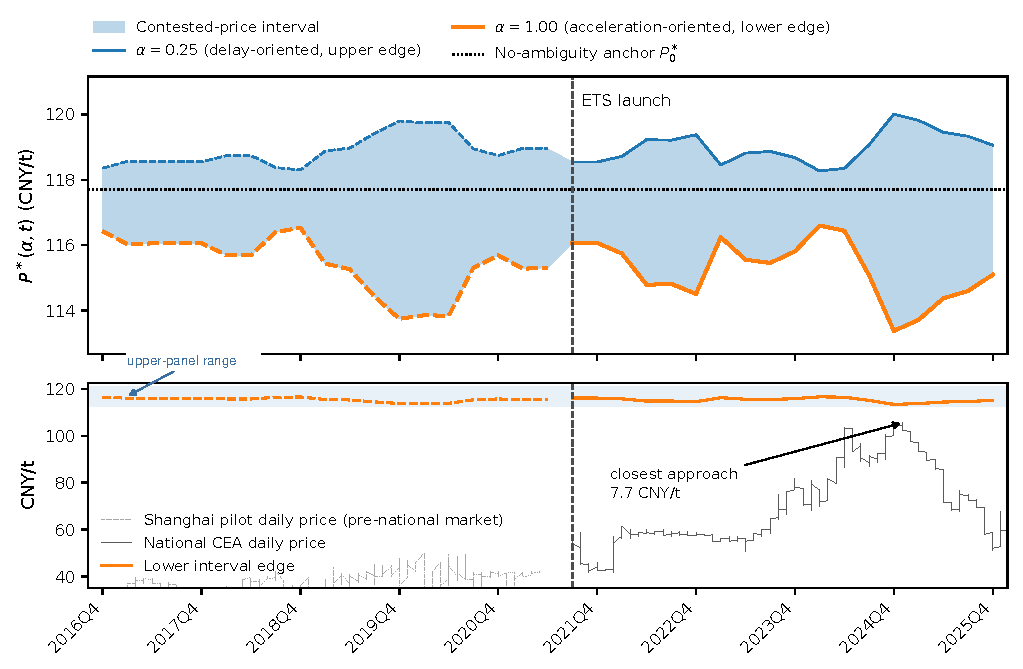
\includegraphics[width=0.9\textwidth]{figures/fig5_dynamic_interval.pdf}
\caption{Retrospective fixed-anchor reconstruction of the contested-price interval for the four-member reference profile. Dashed threshold segments mark the period before the national ETS, and solid segments mark the national ETS period. The vertical dashed line marks the ETS launch, and the horizontal dotted line marks the anchor threshold. The lower panel plots archived daily prices from two markets: the Shanghai pilot price before the national market (dotted) and the national CEA price (solid). The closest-approach annotation compares the lower edge with the national CEA observations only. On the reported path, the lowest lower edge and the highest archived price both fell in 2024Q4, so their difference is the contemporaneous closest approach.}
\label{fig:dynamic}
\end{figure*}

\subsubsection{Archived-price classification}

Under the reference configuration, $\Delta=0$, and the prevailing price equals the archived CEA price. Across the 1,073 daily CEA observations from 2021Q3 to 2025Q4, both the affine rule and the $\aMEU$ benchmark returned unanimous wait. The two rules share the lower interval edge by construction, since the reference profile includes the endpoint weight $\alpha=1$. The highest archived price, 105.65\,CNY/t, lay 7.73\,CNY/t below the lowest member threshold along the reconstructed path. The reference configuration is therefore a nonbinding baseline: retaining the member-threshold vector and its interval left the three-state classification unchanged along this price path. By contrast, changing the radius alone, or one economic primitive alone, produced binding configurations. Of 32 sensitivity configurations evaluated against the same price record, 15 placed the highest archived price at or above the lower edge. Ten of these were released as mixed and four as unanimous invest. The remaining one went to benchmark-model review because the two rules disagreed.

\subsection{Calibration sensitivity and safeguard behavior}

The sensitivity configurations perturb the baseline calibration against the same archived price history, so any change in classification comes from the threshold side.

\subsubsection{Worked gate reports}

Table~\ref{tab:worked} renders two cells of the 32-cell sensitivity design as complete gate reports, which exercise the two branches of the release rule. Both use the lower volatility anchor $\sbar=0.199$, the four-member reference profile, and $V_0=I$, and they differ only in the evaluated radius.

In Configuration A, the radius was the frozen reference peak, and the interval was 4.56\,CNY/t wide. The prevailing price exceeded its upper edge by 0.002\,CNY/t, so all four members classified this price as invest and the gate was unanimous. The member with the smallest recorded weight holds the upper edge, so the edge distance equals the nearest-member distance. This distance of 0.002\,CNY/t was far below the registered envelope of 0.059\,CNY/t. The proximity conditions therefore failed, and the gate issued a dual report after benchmark recomputation. The benchmark placed the upper threshold at 105.60\,CNY/t, against an affine value of 105.65\,CNY/t, and the price cleared both. The proximity rule thus acted conservatively, since the recomputation confirmed unanimous investment. In Configuration B, at the 10\% radius, the interval widened to 7.53\,CNY/t and contained the unchanged prevailing price. Three members classified the price as invest, whereas the member with the smallest recorded weight classified it as wait, so the gate was mixed. Both proximity distances rose to 1.092\,CNY/t, above the envelope of 0.160\,CNY/t, so the affine-only report was released.

In this pair, the wider interval permitted affine-only release, because the release test depends on the distance from the prevailing price to the nearest threshold. Widening carried the upper threshold past the price and raised this distance from 0.002 to 1.092\,CNY/t.

\begin{table*}[!t]
\caption{Worked reports for two cells of the 32-cell sensitivity design, both at the $\sbar=0.199$ calibration.}
\label{tab:worked}
\centering
\footnotesize
\begin{tabular}{@{}lcccc@{}}
\toprule
 & \multicolumn{2}{c}{Configuration A ($\rho=6.057\%$)} & \multicolumn{2}{c}{Configuration B ($\rho=10\%$)}\\
\cmidrule(lr){2-3}\cmidrule(l){4-5}
Report field & Affine & Benchmark & Affine & Benchmark\\
\midrule
\multicolumn{5}{@{}l}{\emph{Member-specific marginal carbon-price thresholds $P^{*}_{i}$ (CNY/t)}}\\
$\alpha_i=0.25$ & 105.65 & 105.60 & 106.74 & 106.62\\
$\alpha_i=0.50$ & 104.13 & 104.07 & 104.23 & 104.07\\
$\alpha_i=0.75$ & 102.61 & 102.56 & 101.73 & 101.60\\
$\alpha_i=1.00$ & 101.09 & 101.09 & 99.22 & 99.22\\
\multicolumn{5}{@{}l}{\emph{Interval, prevailing price, and classification}}\\
Critical weight $\tilde{\alpha}$ (affine) & \multicolumn{2}{c}{0.510} & \multicolumn{2}{c}{0.517}\\
Lower edge of $C_t$ (CNY/t) & 101.09 & 101.09 & 99.22 & 99.22\\
Upper edge of $C_t$ (CNY/t) & 105.65 & 105.60 & 106.74 & 106.62\\
Width $B_t$ (CNY/t) & 4.56 & 4.51 & 7.53 & 7.41\\
Prevailing price $P_t$ (CNY/t) & \multicolumn{2}{c}{105.65} & \multicolumn{2}{c}{105.65}\\
Members classified invest & 4 of 4 & 4 of 4 & 3 of 4 & 3 of 4\\
Gate state & unanimous invest & unanimous invest & mixed & mixed\\
\multicolumn{5}{@{}l}{\emph{Release rule of Eq.~(\ref{eq:safeguard}), evaluated on the affine report}}\\
$\dedge$ (CNY/t) & \multicolumn{2}{c}{0.002} & \multicolumn{2}{c}{1.092}\\
$\dmember$ (CNY/t) & \multicolumn{2}{c}{0.002} & \multicolumn{2}{c}{1.092}\\
Registered envelope $\ER$ (CNY/t) & \multicolumn{2}{c}{0.059} & \multicolumn{2}{c}{0.160}\\
\makecell[l]{Price-recording buffer flag, distance within\\the 1.97\,CNY/t buffer (diagnostic only)} & \multicolumn{2}{c}{unresolved by price record} & \multicolumn{2}{c}{unresolved by price record}\\
Proximity flags & \multicolumn{2}{c}{edge, member} & \multicolumn{2}{c}{none}\\
Reporting mode & \multicolumn{2}{c}{dual report} & \multicolumn{2}{c}{affine-only}\\
Released classification & \multicolumn{2}{c}{unanimous invest} & \multicolumn{2}{c}{mixed}\\
\bottomrule
\end{tabular}
\par\smallskip
\parbox{0.95\textwidth}{\footnotesize\emph{Notes.} The calibration is $r=0.08$, $\mu_c=0.04$, and $\sbar=0.199$, with the reference project value $V_0=I$ and the four-member reference profile. $P_t$ is the highest archived national CEA closing price over 2021Q3 to 2025Q4. Configuration A uses the frozen archived canonical serialized radius key, and its displayed value is rounded for this table only. The upper edge of Configuration A was 105.6481\,CNY/t before rounding, and the prevailing price was 105.65\,CNY/t. The edge therefore lay below the price, although both display as the same rounded value. Edges and widths are rounded independently, so differences of displayed edges can deviate from the displayed width in the last digit. Affine and benchmark thresholds coincide at $\alpha_i=1.00$ by construction. In dual mode, a classification is released only where the two rules agree. In affine-only mode, the benchmark column is shown for comparison.}
\end{table*}

\subsubsection{Margins across the evaluated configurations}

Beyond the two worked cells, Table~\ref{tab:margins} evaluates the baseline calibration, five economic-parameter perturbations, and two additional volatility anchors from Table~\ref{tab:critsens}. For each cell, the table reports the signed margin of each interval edge, defined as the edge minus the highest of the 1,073 archived observations. This price minimizes both signed margins, whereas the release test uses absolute distances, which the highest price need not minimize. A non-positive lower-edge margin means at least one member classifies the price as invest. Unanimous investment also requires a non-positive upper-edge margin, with the price at or above the whole interval.

Under the baseline calibration, the highest archived price entered the interval at the 22\% radius, the upper bound of the primary range. Among the 15 cells with a negative lower-edge margin, both margins were negative in four cells across two rows. Three of these lay in the $r=0.06$ row, where the highest archived price exceeded the upper edge at radii up to 22\%. At the 33\% stress radius, the interval widened enough to contain this price. Two opposing channels shift the threshold level at this discount rate. The smaller characteristic root raises the project-value trigger, whereas the thinner net discount margin lowers the factor converting triggers into prices. The discount-margin channel dominated, so every threshold fell. The fourth cell is Configuration A of Table~\ref{tab:worked}, the lower volatility anchor at the frozen reference-peak radius. Beyond these perturbations, the upper-edge margin also depends on the estimation window of the volatility anchor. The thresholds were recomputed at the reference-peak radius under five national and two pilot windows, with either the relative or the absolute radius held fixed. The archived price stayed outside the interval in every window. The two pilot windows gave a volatility anchor of about 0.95 and thresholds above 500\,CNY/t.

The release rule of Eq.~(\ref{eq:safeguard}) raised an edge or member proximity flag in five of the 32 cells. Four of these lay at the 22\% and 33\% radii, where the mandatory wide-radius branch already covers all 16 cells. The fifth was Configuration A of Table~\ref{tab:worked}. The 16 mandatory cells and this flagged cell gave 17 benchmark fallbacks. These fallbacks captured every disagreement between the two rules across the 32 cells. One gate-state disagreement occurred at the 33\% radius under $r=0.06$, where the affine rule reported a mixed gate and the benchmark reported unanimous invest. Two member-label disagreements also occurred. A separate diagnostic uses the 1.97\,CNY/t price-recording buffer, which represents the recording granularity of the archived price series. Six of the 32 cells placed the highest archived price within this buffer of an interval edge. Three of these six cells were among the five flagged cells.

\begin{table*}[!t]
\caption{Signed margin of each edge of the contested-price interval relative to the highest archived carbon price. The configurations are the economic perturbations and volatility anchors of the sensitivity analysis. SHEA denotes the Shanghai Emission Allowance pilot market.}
\label{tab:margins}
\centering
\footnotesize
\setlength{\tabcolsep}{4pt}
\begin{tabular}{@{}lcccccccc@{}}
\toprule
 & \multicolumn{4}{c}{Margin to the lower edge (CNY/t)} & \multicolumn{4}{c}{Margin to the upper edge (CNY/t)}\\
\cmidrule(lr){2-5}\cmidrule(l){6-9}
Configuration at $h/\sbar$ & 6.057\% & 10\% & 22\% & 33\% & 6.057\% & 10\% & 22\% & 33\%\\
\midrule
Baseline calibration & $+7.7$ & $+5.0$ & $-2.8$ & $-9.3$ & $+14.4$ & $+16.0$ & $+21.3$ & $+26.8$\\
$r=0.06$ ($-25\%$) & $-16.8$ & $-19.3$ & $-26.2$ & $-31.9$ & $-10.8$ & $-9.4$ & $-4.4$ & $+0.9$\\
$r=0.12$ ($+50\%$) & $+55.0$ & $+51.9$ & $+42.7$ & $+34.9$ & $+62.7$ & $+64.5$ & $+70.4$ & $+76.4$\\
$\mu_c=0.06$ ($+50\%$) & $+0.5$ & $-1.9$ & $-8.7$ & $-14.2$ & $+6.5$ & $+8.0$ & $+13.0$ & $+18.3$\\
$\sbar=0.199$ ($-20\%$) & $-4.6$ & $-6.4$ & $-11.8$ & $-16.3$ & $-0.0019$ & $+1.1$ & $+4.7$ & $+8.5$\\
$\sbar=0.299$ ($+20\%$; early CEA anchor regime) & $+21.8$ & $+18.1$ & $+7.5$ & $-1.2$ & $+30.9$ & $+33.1$ & $+40.4$ & $+48.1$\\
Pooled national, 2021Q3 to 2025Q4 ($\sbar=0.278$) & $+15.7$ & $+12.4$ & $+3.0$ & $-4.7$ & $+23.7$ & $+25.6$ & $+32.1$ & $+38.8$\\
SHEA pilot, 2016 to 2021Q1 ($\sbar=0.953$) & $+376.9$ & $+345.6$ & $+258.3$ & $+188.5$ & $+455.1$ & $+474.7$ & $+542.3$ & $+614.9$\\
\bottomrule
\end{tabular}
\par\smallskip
\parbox{0.97\textwidth}{\footnotesize\emph{Notes.} Each margin is the stated interval edge minus the highest archived national CEA closing price over 2021Q3 to 2025Q4 (105.65\,CNY/t, 1,073 observations). A positive lower-edge margin means every member classifies every archived price as wait. A negative lower-edge margin with a positive upper-edge margin means a mixed gate. When both margins are negative, every member classifies the price as invest. The radius is fixed within each column. The 6.057\% value is the displayed peak of the reconstructed signal path. This radius uses the frozen archived canonical serialized key, and its displayed value is rounded for the table only. The 10\% radius is the affine-only cap, 22\% is the upper bound of the primary radius range, and 33\% is the stress radius. Classifications and release decisions use unrounded values. A margin below 0.05\,CNY/t in absolute value is shown at four decimals, so its sign remains legible. At a given radius, the upper-edge margin minus the lower-edge margin equals the interval width up to rounding. It equaled 6.63\,CNY/t only in the baseline row at the reference-peak radius. Each configuration matches the corresponding row of Table~\ref{tab:critsens}. The underlying edge values are in data/observed\_margin\_both\_edges.csv of the replication archive.}
\end{table*}
